\chapter[Resultados Alcançados]{\textbf{R}esultados \textbf{A}lcançados}
%\addcontentsline{toc}{chapter}{Resultados Alcançados}

\textit{Será apresentado neste capítulo a execução dos experimentos sob a solução abordada nas seções anteriores, e exposto os resultados que foram alcançados.}

\section{Materiais e Métodos}

Os experimentos sobre a solução de integração dos sistemas, foram necessários grandes esforços tanto no planejamento de um ambiente controlado quanto na elaboração e análise dos cenários de testes envolvidos. Para que os cenários de teste sejam o mais semelhante ao ambiente de produção os mesmo serão executados sobre uma chamada telefônica tendo como originador o suposto cliente com as devidas características. 

\subsection{Ambiente de teste}

O ambiente para execução dos testes será realizando um terminal cujo as especificações estão descritas abaixo:

\begin{table}[htb]
	\footnotesize
	\caption{Recursos computacionais utilizados}
	\label{tabela:recursosUtilizados}
	\begin{tabular}{|p{3.5cm}|p{3cm}|p{2cm}|p{4cm}|} \hline
		\textbf{SISTEMA OPER.} 	& \textbf{PROCESSADOR} 				& \textbf{MEMÓRIA} 	& \textbf{ARMAZENAMENTO}  \\ \hline
		Windows 7 64 bits 		& Intel Core i7-3520M CPU@2.9GHz 	& 8GB DDR3			& 1TB 5400 rpm \\ \hline
	\end{tabular}
	\legend{\fontsize{10}{12}\selectfont {Fonte: Autoria Própria}.}
\end{table}

Este terminal é responsável em executar ambos os sistemas envolvidos, no entanto como software Asterisk está disponível somente para plataforma Linux será utilizado o recurso de máquina virtual através do software Virtual Box\footnote{Disponível em \url{https://www.virtualbox.org/}}, para subir uma instância da distribuição Disc-Os conforme citado nas seções anteriores.
 
O terminal possui uma conexão de rede local ativa, para que seja atribuído uma faixa de IP ao sistema operacional hospedeiro e ao convidado.
Visando garantir o correto funcionamento e a padronização do ambiente de teste foram criados testes de integração reproduzindo uma chamada telefônica programaticamente simulando um ambiente real, para tanto foi necessário utilizar os seguintes recursos o framework JUnit na construção dos testes e o recurso nativo do Asterisk chamado \textit{Local Channel} que permite criar um canal de comunicação com um contexto e extensão específica dentro do sistema Asterisk, ou seja permite acessar diretamente o ponto de integração entre os sistemas.

Foram criados contextos específicos para teste no software Asterisk, conforme visto abaixo;

\begin{figure}[H]
	\centering
	\caption{Contexto de Teste}
	\label{figura:contextoTeste}
	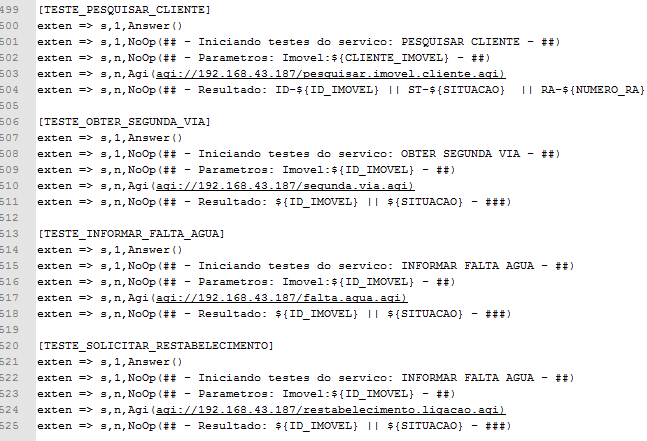
\includegraphics{figuras/contexto_teste.png}
	\legend {\fontsize{10}{12}\selectfont {Fonte: Autoria Própria}.}	
\end{figure}



\subsection{Elaboração dos Cenários de Teste}

Os cenários de testes representam as possíveis situações cadastrais vinculadas a um cliente ou imóvel necessários para realizar um atendimento via sistema. Foram propostos 4 cenários de teste para cada serviço automatizado, visando assegurar o correto comportamento da solução. Abaixo estão descritos os cenários conforme cada serviços proposto:

\subsubsection{Obter 2ª Via de Conta}
Abaixo serão descritos os casos de testes previstos para o serviço Obter 2ª Via de Conta.
\begin{flushleft}
	\begin{description}
		\item \textbf{CENÁRIO 1}: Cliente devidamente cadastrado no Sistema, atualmente proprietário de um único imóvel que possui ativo a Ligação de Água e Esgoto, com pendência de duas contas. O Cliente deseja obter as duas contas em aberto.
	\end{description}
	
	\begin{description}
		\item \textbf{CENÁRIO 2}: Cliente devidamente cadastrado no Sistema, atualmente sendo usuário de um imóvel que possui a Ligação de Água cortada por falta de pagamento, atualmente com quatro contas em aberto. O Cliente deseja obter as quatro contas em aberto.
	\end{description}
	
	\begin{description}
		\item \textbf{CENÁRIO 3}: Cliente devidamente cadastrado no Sistema, atualmente sendo responsável por três imóveis que possuem ativo a Ligação de Água e Esgoto, possuindo uma conta pendente para cada imóvel. O Cliente pretende obter a conta pendente de somente um imóvel específico. 
	\end{description}
	
	\begin{description}
		\item \textbf{CENÁRIO 4}: Cliente sem e-mail cadastrado no Sistema, atualmente sendo responsável por dois imóveis que possuem ativo a Ligação de Água e Esgoto, possuindo duas contas pendente para cada imóvel.  O cliente pretende obter todas a contas em aberto dos dois imóveis. 
	\end{description}
\end{flushleft}


\subsubsection{Informar Falta de Água}
Abaixo serão descritos os casos de testes previstos para o serviço Informar Falta de Água.
\begin{flushleft}
	\begin{description}
		\item \textbf{CENÁRIO 1}: Cliente devidamente cadastrado no Sistema, atualmente proprietário de um único imóvel que possui ativo a Ligação de Água e Esgoto, com pendência de duas contas, com problemas no abastecimento de água. O Cliente pretende informar a falta de água para o único imóvel.
	\end{description}
	\begin{description}
		\item \textbf{CENÁRIO 2}: Cliente sem e-mail cadastrado no Sistema, atualmente usuário de um único imóvel que possui ativo a Ligação de Água, com situação de adimplência, com problemas no abastecimento de água. O Cliente pretende informar a falta de água para o único imóvel.
	\end{description}
	\begin{description}
		\item \textbf{CENÁRIO 3}: Cliente devidamente cadastrado no Sistema, atualmente responsável por três imóveis que possuem ativo a Ligação de Água, com uma conta pendente para cada imóvel. O Cliente deseja informar problemas no abastecimento de água para um imóvel específico ao qual o mesmo é responsável.
	\end{description}
	\begin{description}
		\item \textbf{CENÁRIO 4}: Cliente devidamente cadastrado no Sistema, atualmente responsável por dois imóveis em locais diferentes, que possuem a Ligação de Água ativa, em recente situação de adimplência. O Cliente deseja informar problemas no abastecimento de água para os dois imóveis ao qual o mesmo é responsável.
	\end{description}
\end{flushleft}	

\subsubsection{Solicitar Restabelecimento da Ligação de Água}
Abaixo serão descritos os casos de testes previstos para o serviço Solicitar Restabelecimento da Ligação de Água.
\begin{flushleft}
	\begin{description}
		\item \textbf{CENÁRIO 1}: Cliente devidamente cadastrado no Sistema, atualmente proprietário de um único imóvel que possui a Ligação de Água interrompida por corte, em situação recente de adimplência. O Cliente deseja solicitar restabelecimento da ligação para o imóvel.
	\end{description}
	\begin{description}
		\item \textbf{CENÁRIO 2}: Cliente devidamente cadastrado no Sistema, atualmente usuário de um único imóvel que possui a Ligação de Água interrompida por corte, em situação recente de adimplência. O Cliente deseja solicitar restabelecimento da ligação para o imóvel.
	\end{description}
	\begin{description}
		\item \textbf{CENÁRIO 3}: Cliente devidamente cadastrado no Sistema, atualmente responsável por dois imóveis, que possuem a Ligação de Água interrompida por corte, devido a falta de pagamento das dez contas em aberto para ambos. O Cliente deseja solicitar restabelecimento da ligação para os imóveis após realizar a negociação das faturas.
	\end{description}
	
	\begin{description}
		\item \textbf{CENÁRIO 4}: Cliente com cadastrado incompleto no Sistema, atualmente proprietário de um único imóvel que possui a Ligação de Água interrompida por corte, em situação recente de adimplência. O Cliente deseja solicitar restabelecimento da ligação para o imóvel.
	\end{description}
\end{flushleft}	


\subsection{Execução dos Cenários de Teste}
A execução dos cenários propostos será realizada utilizando 
Os cenários de testes representam as possíveis situações cadastrais ou comportamentais apresentadas pelo cliente ao longo do atendimento, onde cada cenário deve ser totalmente atendimento para que se tenha êxito no atendimento e posteriormente a situação de \textbf{ATENDINDO}, caso contrário será obtido à situação de \textbf{NÃO ATENDINDO}, caso o atendimento não seja concluído com sucesso o cenário deve conter uma observação, descrevendo o motivo ao qual levou a tal situação.
Abaixo serão descritos os Cenários dos serviços propostos:


\subsubsection{Obter 2ª Via de Conta}
Abaixo serão descritos os casos de testes previstos para o serviço Obter 2ª Via de Conta;
\begin{flushleft}
	\begin{description}
		\item \textbf{CENÁRIO 1}: Cliente devidamente cadastrado no Sistema, atualmente proprietário de um único imóvel que possui ativo a Ligação de Água e Esgoto, com pendência de duas contas. O Cliente deseja obter as duas contas em aberto.
		\item \textbf{SITUAÇÃO}: ATENDINDO
		\item \textbf{OBSERVAÇÃO}: Não aplicável
	\end{description}
	
	\begin{description}
		\item \textbf{CENÁRIO 2}: Cliente devidamente cadastrado no Sistema, atualmente sendo usuário de um imóvel que possui a Ligação de Água cortada por falta de pagamento, atualmente com quatro contas em aberto. O Cliente deseja obter as quatro contas em aberto.
		\item \textbf{SITUAÇÃO}: ATENDINDO
		\item \textbf{OBSERVAÇÃO}: Não aplicável
	\end{description}
	
	\begin{description}
		\item \textbf{CENÁRIO 3}: Cliente devidamente cadastrado no Sistema, atualmente sendo responsável por três imóveis que possuem ativo a Ligação de Água e Esgoto, possuindo uma conta pendente para cada imóvel. O Cliente pretende obter a conta pendente de somente um imóvel específico. 
		\item \textbf{SITUAÇÃO}: ATENDINDO
		\item \textbf{OBSERVAÇÃO}: Não aplicável
	\end{description}
	
	\begin{description}
		\item \textbf{CENÁRIO 4}: Cliente sem e-mail cadastrado no Sistema, atualmente sendo responsável por dois imóveis que possuem ativo a Ligação de Água e Esgoto, possuindo duas contas pendente para cada imóvel.  O cliente pretende obter todas a contas em aberto dos dois imóveis. 
		\item \textbf{SITUAÇÃO}: NÃO ATENDINDO
		\item \textbf{OBSERVAÇÃO}: Devido a falta do e-mail no cadastro do cliente não será possível enviar as contas pendentes ao mesmo, e também a solução inicialmente está tratando dos débitos de um imóvel por vez, sendo necessário redirecionar a ligação para o atendente concluir o atendimento, ou repetir a operação.
	\end{description}
\end{flushleft}


\subsubsection{Informar Falta de Água}
Abaixo serão descritos os casos de testes previstos para o serviço Informar Falta de Água;
\begin{flushleft}
	\begin{description}
		\item \textbf{CENÁRIO 1}: Cliente devidamente cadastrado no Sistema, atualmente proprietário de um único imóvel que possui ativo a Ligação de Água e Esgoto, com pendência de duas contas, com problemas no abastecimento de água. O Cliente pretende informar a falta de água para o único imóvel.
		\item \textbf{SITUAÇÃO}: ATENDINDO
		\item \textbf{OBSERVAÇÃO}: Não aplicável
	\end{description}
	\begin{description}
		\item \textbf{CENÁRIO 2}: Cliente sem e-mail cadastrado no Sistema, atualmente usuário de um único imóvel que possui ativo a Ligação de Água, com situação de adimplência, com problemas no abastecimento de água. O Cliente pretende informar a falta de água para o único imóvel.
		\item \textbf{SITUAÇÃO}: ATENDINDO
		\item \textbf{OBSERVAÇÃO}: Não aplicável
	\end{description}
	\begin{description}
		\item \textbf{CENÁRIO 3}: Cliente devidamente cadastrado no Sistema, atualmente responsável por três imóveis que possuem ativo a Ligação de Água, com uma conta pendente para cada imóvel. O Cliente deseja informar problemas no abastecimento de água para um imóvel específico ao qual o mesmo é responsável.
		\item \textbf{SITUAÇÃO}: ATENDINDO
		\item \textbf{OBSERVAÇÃO}: Não aplicável
	\end{description}
	\begin{description}
		\item \textbf{CENÁRIO 4}: Cliente devidamente cadastrado no Sistema, atualmente responsável por dois imóveis em locais diferentes, que possuem a Ligação de Água ativa, em recente situação de adimplência. O Cliente deseja informar problemas no abastecimento de água para os dois imóveis ao qual o mesmo é responsável.
		\item \textbf{SITUAÇÃO}: NÃO ATENDINDO
		\item \textbf{OBSERVAÇÃO}: A solução inicialmente para Informar Falta de Água está tratando apenas um imóvel por vez, sendo necessário redirecionar a ligação para o atendente concluir o atendimento, ou repetir a operação.
	\end{description}
\end{flushleft}	

\subsubsection{Solicitar Restabelecimento da Ligação de Água}
Abaixo serão descritos os casos de testes previstos para o serviço Solicitar Restabelecimento da Ligação de Água;
\begin{flushleft}
	\begin{description}
		\item \textbf{CENÁRIO 1}: Cliente devidamente cadastrado no Sistema, atualmente proprietário de um único imóvel que possui a Ligação de Água interrompida por corte, em situação recente de adimplência. O Cliente deseja solicitar restabelecimento da ligação para o imóvel.
		\item \textbf{SITUAÇÃO}: ATENDINDO
		\item \textbf{OBSERVAÇÃO}: Não aplicável
	\end{description}
	\begin{description}
		\item \textbf{CENÁRIO 2}: Cliente devidamente cadastrado no Sistema, atualmente usuário de um único imóvel que possui a Ligação de Água interrompida por corte, em situação recente de adimplência. O Cliente deseja solicitar restabelecimento da ligação para o imóvel.
		\item \textbf{SITUAÇÃO}: ATENDINDO
		\item \textbf{OBSERVAÇÃO}: Não aplicável
	\end{description}
	\begin{description}
		\item \textbf{CENÁRIO 3}: Cliente devidamente cadastrado no Sistema, atualmente responsável por dois imóveis, que possuem a Ligação de Água interrompida por corte, devido a falta de pagamento das dez contas em aberto para ambos. O Cliente deseja solicitar restabelecimento da ligação para os imóveis após realizar a negociação das faturas.
		\item \textbf{SITUAÇÃO}: NÃO ATENDINDO
		\item \textbf{OBSERVAÇÃO}: A solução inicialmente está tratando o restabelecimento da ligação de apenas um imóvel por vez, sendo necessário redirecionar a ligação para o atendente concluir o atendimento, ou repetir a operação.
	\end{description}
	
	\begin{description}
		\item \textbf{CENÁRIO 4}: Cliente com cadastrado incompleto no Sistema, atualmente proprietário de um único imóvel que possui a Ligação de Água interrompida por corte, em situação recente de adimplência. O Cliente deseja solicitar restabelecimento da ligação para o imóvel.
		\item \textbf{SITUAÇÃO}: ATENDINDO
		\item \textbf{OBSERVAÇÃO}: Não aplicável	
	\end{description}
\end{flushleft}	